\documentclass[12pt]{article}

\usepackage{a4wide}
\usepackage{enumerate}
\usepackage{fontspec}
\usepackage[]{hyperref}
\hypersetup{
  colorlinks=true,
  linkcolor=blue,
  urlcolor=blue
}
\usepackage{tikz}
\tikzstyle{vertex}=[circle,fill=black!25,minimum size=20pt,inner sep=0pt]
\tikzstyle{selected vertex} = [vertex, fill=blue!24]
\tikzstyle{edge} = [draw,thick,->,bend left]
\tikzstyle{weight} = [font=\small]
\tikzstyle{selected edge} = [draw,line width=5pt,-,red!50]
\tikzstyle{ignored edge} = [draw,line width=5pt,-,black!20]
\usepackage{tkz-berge}

\begin{document}
\title{Grafos: caminhos mínimos}
\author{Adriano J. Holanda, Zhao Liang}
\date{\today}
\maketitle

\section*{Algoritmo de Dijkstra usando lista de adjacências}

\paragraph{1.}~Compare o código fonte contendo a declaração da
estrutura de dados para o grafo usando lista de adjacências e a
implementação do algoritmo de Dijkstra com o código apresentado em
sala de aula.
\begin{enumerate}[a)]
\item Verifique o que estava faltando.
\item Por quê não há mais necessidade da variável {\tt visitado[]}?
\item Qual o valor da constante {\tt INFINITO}? Por quê não é {\tt
  LONG\_MAX}?
\item Como é inserido um vértice no grafo?
\item Como é inserido um arco no grafo?
\item Qual alteração deveria ser feita para tornar o grafo
  não-direcionado?
\end{enumerate}

\paragraph{2.} Complete a implementação do algoritmo de Dijstra
\href{https://drive.google.com/open?id=1yHk413g7MF2NU4v6MqLlEQrrmnYkfVU9}{dijkstra\_fila.c}
com as instruções que estão faltando.

\pagebreak
\paragraph{3.} Para os grafos a seguir:

\begin{enumerate}[a)]
\item Aplique o algoritmo de Dijstra no grafo utilizando caneta/lápis
  e papel e mostrando os valores intermediários para a fila de
  prioridade e finais para o campo {\tt precede}~\footnote{O campo
    {\tt precede} também é chamado de {\tt predecessor} ou {\tt prev}
    em alguns livros didáticos} de cada vértice.

\item Crie o grafo usando o programa preenchido no exercício 2 e
  execute o algoritmo de Dijkstra em cada grafo.

\end{enumerate}

\begin{enumerate}[i)]

\item {\tt dijkstra(0, 3);}
\begin{center}
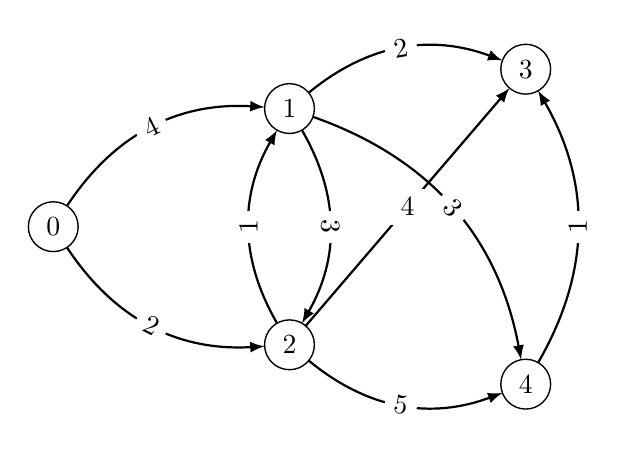
\begin{tikzpicture}[transform shape]
  \centering
  \Vertex[x=-3,y=0]{0}
  \Vertex[x=0,y=1.5]{1}
  \Vertex[x=0,y=-1.5]{2}
  \Vertex[x=3,y=2]{3}
  \Vertex[x=3,y=-2]{4}
  \tikzstyle{EdgeStyle}=[->,>=latex]
  \Edge[label=$4$](2)(3)
  \tikzstyle{LabelStyle}=[fill=white,sloped]
  \tikzstyle{EdgeStyle}=[->,>=latex,bend left]
  \Edge[label=$4$](0)(1)
  \Edge[label=$3$](1)(2)
  \Edge[label=$2$](1)(3)
  \Edge[label=$3$](1)(4)
  \Edge[label=$1$](2)(1)
  \tikzstyle{EdgeStyle}=[->,>=latex,bend right]
  \Edge[label=$2$](0)(2)
  \Edge[label=$5$](2)(4)
  \Edge[label=$1$](4)(3)
  \label{fig:dijk03}
\end{tikzpicture}
\end{center}

\item {\tt dijkstra(0, 5);}

  \begin{center}
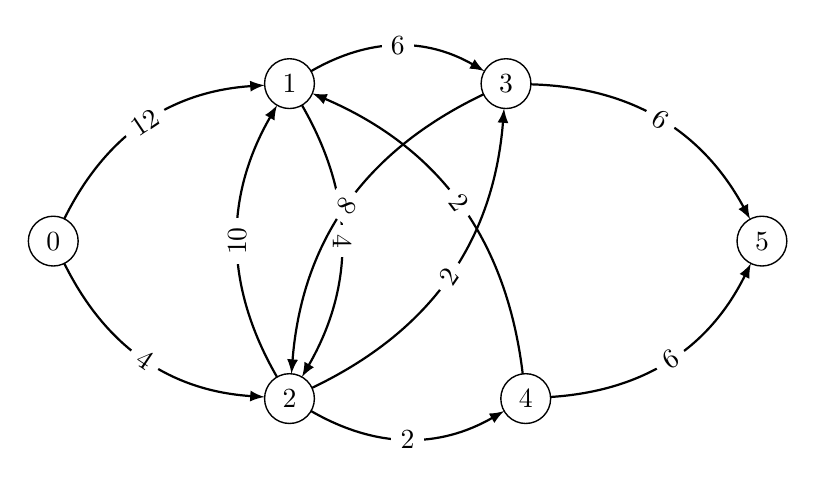
\begin{tikzpicture}[transform shape]
  \centering
  \Vertex[x=-3,y=0]{0}
  \Vertex[x=0,y=2]{1}
  \Vertex[x=0,y=-2]{2}
  \Vertex[x=2.75,y=2]{3}
  \Vertex[x=3,y=-2]{4}
  \Vertex[x=6,y=0]{5}
  \tikzstyle{LabelStyle}=[fill=white,sloped]
  \tikzstyle{EdgeStyle}=[->,>=latex,bend left]
  \Edge[label=$12$](0)(1)
  \Edge[label=$4$](1)(2)
  \Edge[label=$6$](1)(3)
  \Edge[label=$10$](2)(1)
  \Edge[label=$6$](3)(5)
  \tikzstyle{EdgeStyle}=[->,>=latex,bend right]
  \Edge[label=$2$](2)(3)
  \Edge[label=$4$](0)(2)
  \Edge[label=$2$](2)(4)
  \Edge[label=$8$](3)(2)
  \Edge[label=$2$](4)(1)
  \Edge[label=$6$](4)(5)
  \label{fig:dijk05}
\end{tikzpicture}
\end{center}

\end{enumerate}


\end{document}

\section*{Algoritmo de Dijkstra usando matriz de adjacências}

\paragraph{1.}~Compare o código fonte contendo a declaração da
estrutura de dados para o grafo usando matriz de adjacências e a
implementação do algoritmo de Dijkstra com o código apresentado em
sala de aula.
\begin{enumerate}[a)]
\item Verifique o que estava faltando.
\item Como o grafo foi declarado.
\item Se há alocação de memória, se não há, qual mecanismo é utilizado
  para utilização da estrutura grafo?
\item Onde está a matriz de adjacência e como é inicializada.
\item Onde estão as variáveis {\tt dist[]}, {\tt visitado[]} e {\tt
    precede[]} e como são inicializadas. Por quê estão declaradas na
  estrutura grafo?
\item Qual o valor da constante {\tt INFINITO}?
\item Como o número de elementos da matriz de adjacências pode ser
  aumentado?
\item Como é inserido um vértice no grafo?
\item Como é inserido um arco no grafo?
\item Qual alteração deveria ser feita para tornar o grafo
  não-direcionado?
\item O algoritmo de Dijkstra também pode ser aplicado a grafos não
  direcionados?
\end{enumerate}

\paragraph{2.} A implementação do algoritmo de Dijkstra usando matriz
de adjacências não segue estritamente o enunciado original do
algoritmo. Explique o motivo e como este detalhe é contornado.

\pagebreak
\paragraph{3.} Carregue os seguintes grafos e verifique, cuidadosamente,
as tabelas intermediárias geradas.

\begin{enumerate}[a)]

\item {\tt dijkstra(0, 3);}
\begin{center}
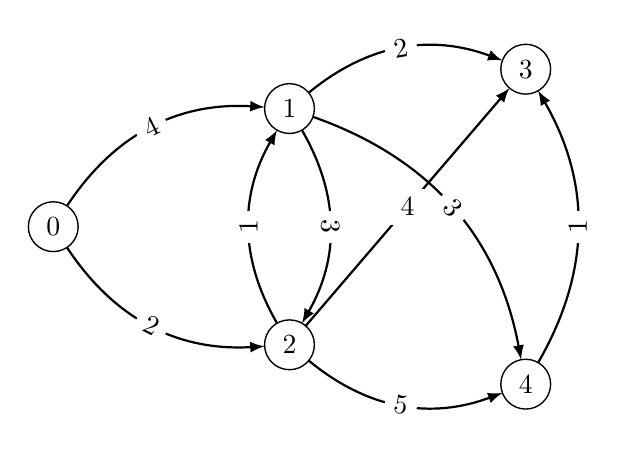
\begin{tikzpicture}[transform shape]
  \centering
  \Vertex[x=-3,y=0]{0}
  \Vertex[x=0,y=1.5]{1}
  \Vertex[x=0,y=-1.5]{2}
  \Vertex[x=3,y=2]{3}
  \Vertex[x=3,y=-2]{4}
  \tikzstyle{EdgeStyle}=[->,>=latex]
  \Edge[label=$4$](2)(3)
  \tikzstyle{LabelStyle}=[fill=white,sloped]
  \tikzstyle{EdgeStyle}=[->,>=latex,bend left]
  \Edge[label=$4$](0)(1)
  \Edge[label=$3$](1)(2)
  \Edge[label=$2$](1)(3)
  \Edge[label=$3$](1)(4)
  \Edge[label=$1$](2)(1)
  \tikzstyle{EdgeStyle}=[->,>=latex,bend right]
  \Edge[label=$2$](0)(2)
  \Edge[label=$5$](2)(4)
  \Edge[label=$1$](4)(3)
  \label{fig:dijk03}
\end{tikzpicture}
\end{center}

\item {\tt dijkstra(0, 5);}

  \begin{center}
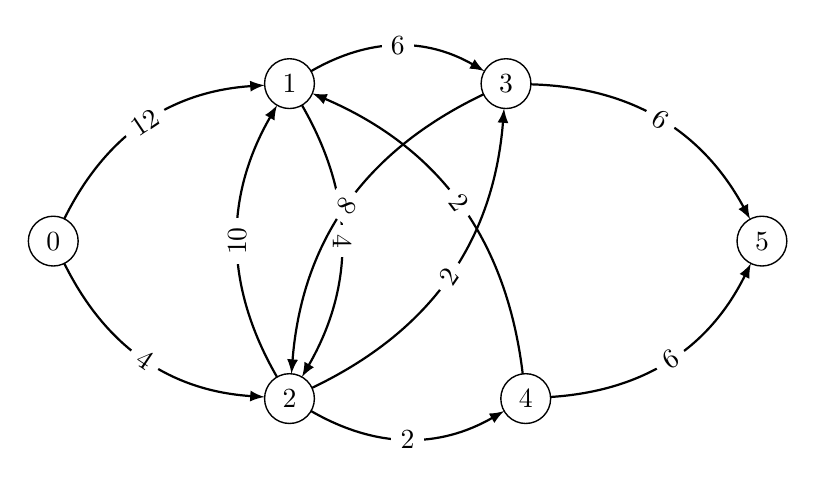
\begin{tikzpicture}[transform shape]
  \centering
  \Vertex[x=-3,y=0]{0}
  \Vertex[x=0,y=2]{1}
  \Vertex[x=0,y=-2]{2}
  \Vertex[x=2.75,y=2]{3}
  \Vertex[x=3,y=-2]{4}
  \Vertex[x=6,y=0]{5}
  \tikzstyle{LabelStyle}=[fill=white,sloped]
  \tikzstyle{EdgeStyle}=[->,>=latex,bend left]
  \Edge[label=$12$](0)(1)
  \Edge[label=$4$](1)(2)
  \Edge[label=$6$](1)(3)
  \Edge[label=$10$](2)(1)
  \Edge[label=$6$](3)(5)
  \tikzstyle{EdgeStyle}=[->,>=latex,bend right]
  \Edge[label=$2$](2)(3)
  \Edge[label=$4$](0)(2)
  \Edge[label=$2$](2)(4)
  \Edge[label=$8$](3)(2)
  \Edge[label=$2$](4)(1)
  \Edge[label=$6$](4)(5)
  \label{fig:dijk05}
\end{tikzpicture}
\end{center}

\item {\tt dijkstra(0, 7);}

  \begin{center}
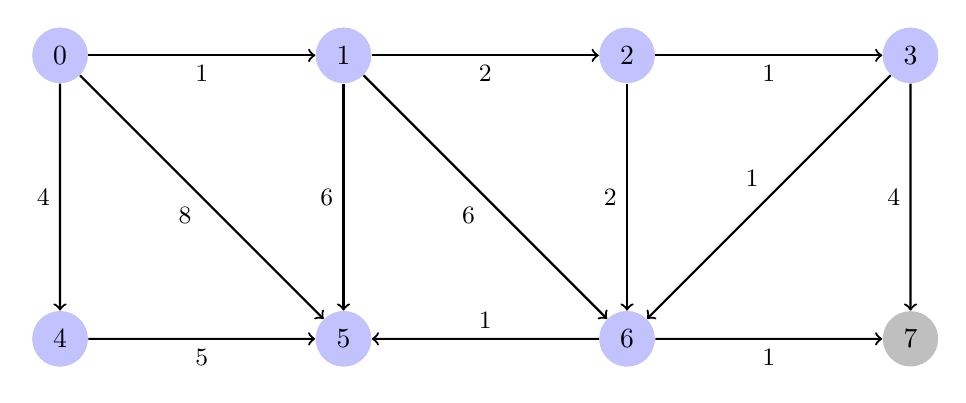
\begin{tikzpicture}[scale=1.8, auto,swap]
  \centering
    % Draw a 7,11 network
    % First we draw the vertices
    \foreach \pos/\name in {{(-3,0)/0},{(-1,0)/1},{(1,0)/2},{(3,0)/3},
                            {(-3,-2)/4},{(-1,-2)/5},{(1,-2)/6},{(3,-2)/7}}
        \node[vertex] (\name) at \pos {$\name$};
    % Connect vertices with edges and draw weights
        \foreach \source/ \dest /\weight in {
          0/1/1,0/4/4,0/5/8,
          1/2/2,1/5/6,1/6/6,
          2/3/1,2/6/2,
          3/6/1,3/7/4,
          4/5/5,
          6/5/1,6/7/1}
        \path[edge] (\source) -- node[weight] {$\weight$} (\dest);
    % Start animating the vertex and edge selection.
    \foreach \vertex / \fr in {0/1,1/2,2/3,3/4,4/5,5/6,6/7}
    \path node[selected vertex] at (\vertex) {$\vertex$};
  \label{fig:dijk07}
\end{tikzpicture}
\end{center}

\end{enumerate}

\end{document}
